%%%%%%%%%%%%%%%%%%%%%%%%%%%%%%%%%%%%%%%%%%%%%%%%%%%%%%%%%%%%%%%%%%%%%%%%%%%%%%%%%%%%
% Document data
%%%%%%%%%%%%%%%%%%%%%%%%%%%%%%%%%%%%%%%%%%%%%%%%%%%%%%%%%%%%%%%%%%%%%%%%%%%%%%%%%%%%
\documentclass[12pt]{article} %report allows for chapters
%%%%%%%%%%%%%%%%%%%%%%%%%%%%%%%%%%%%%%%%%%%%%%%%%%%%%%%%%%%%%%%%%%%%%%%%%%%%%%%%%%%%
\usepackage{preamble}

\begin{document}

\begin{center}
   \textsc{\large MATH 271, Worksheet 1}\\
   \textsc{Complex Numbers}
\end{center}
\vspace{.5cm}

\begin{problem}
Add and multiply all possible pairs of the complex numbers
\[
z_1 = 3-2i \qquad z_2 = -1-i \qquad z_3 = \frac{1}{\sqrt{2}}+\frac{i}{\sqrt{2}} \qquad z_4 = -\pi + \pi i.
\]
\end{problem}

\begin{problem}
Plot and label the above points on the graph below. Pick two points and draw their sum geometrically. 
        \begin{center}
        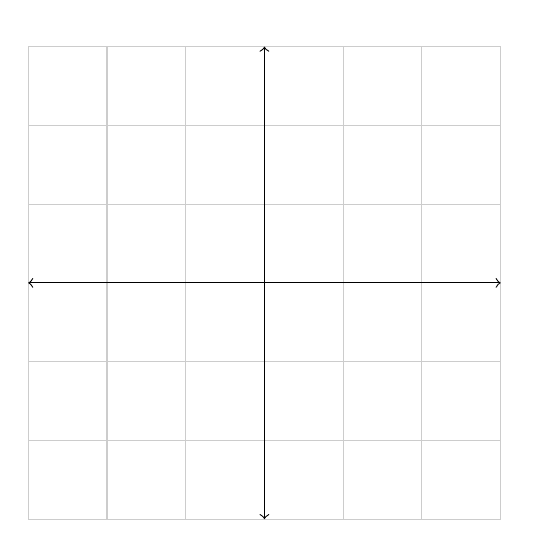
\begin{tikzpicture}
        \draw[thin,gray!40] (-3,-3) grid (3,3);
        \draw[<->] (-3,0)--(3,0) node[right]{$\RE$};
        \draw[<->] (0,-3)--(0,3) node[above]{$\IM$};
        \end{tikzpicture}
        \end{center}
\end{problem}

\begin{problem}
Convert all the above complex numbers in Cartesian form to polar form.
\end{problem}

\begin{problem}
Multiply all possible pairs of complex numbers
\[
w_1 = e^{i\pi} \qquad w_2 = -\sqrt{2} e^{i\frac{\pi}{4}} \qquad w_3 = 2 e^{-i\frac{\pi}{3}} \qquad w_4= 3 e^{i\frac{\pi}{2}}.
\]
\end{problem}

\begin{problem}
Plot and label the above points in the graph below.  Draw the product $w_1w_2$ geometrically.
        \begin{center}
        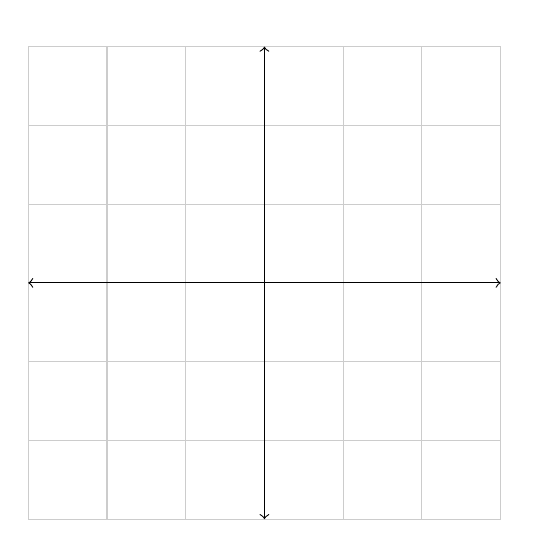
\begin{tikzpicture}
        \draw[thin,gray!40] (-3,-3) grid (3,3);
        \draw[<->] (-3,0)--(3,0) node[right]{$\RE$};
        \draw[<->] (0,-3)--(0,3) node[above]{$\IM$};
        \end{tikzpicture}
        \end{center}
\end{problem}
\newpage

\begin{problem}
Show by a geometrical argument that $re^{i\theta}=re^{i(\theta+2n\pi)}$ for any integer value of $n$.  Can you also show this by the typical conversion from polar to Cartesian?
\end{problem}

\begin{problem}
Let $z=a+bi$.  What is $z^*?$  What is $z$ in polar coordinates? How about $z^*$? Can you explain why $zz^*$ will always be real using a geometrical (polar coordinate) argument?
\end{problem}

\begin{problem}
Show that the functions $\sin(x)$ and $\cos(x)$ are periodic and determine the period.  Is the function $\tan(x)$ periodic?
\end{problem}

\begin{problem}
(Roots of unity) Given that $i^2=-1$ we can factor equations in ways that are totally new to us.  Solve the following. Geometrical reasoning may really help you here!
\begin{enumerate}[(a)]
    \item Find all solutions to $z^2=1$.
    \item Find all solutions to $z^3=1$.
    \item Find all solutions to $z^4=1$.
    \item *Find all solutions to $z^n=1$.
\end{enumerate}
\emph{Hint: each of the above has $n$ solutions for $z^n$.}
\end{problem}

\begin{problem}
(Rotational symmetries) Consider a complex number $z=a+bi=re^{i\theta}$. What happens to this point as we repeatedly multiply by $i$? Pick a specific $z$ (i.e., fix $a$ and $b$ or $r$ and $\theta$) and multiply by $i$ until you see a pattern.  What is happening? \emph{Note: this is an example of a symmetry group or a discrete dynamical system!}
\end{problem}

\begin{problem}
(Why $i$?) Consider the following (differential) equation
\[
\frac{d^2}{dt^2}x(t)=-x(t).
\]
Now, let $x(t)=e^{it}$.  Show that the above expression is true.
\end{problem}

\begin{problem}
(Characteristic polynomial) Consider the following (differential) equation
\[
ax''(t)+bx'(t)+cx(t)=0.
\]
This equation can be converted to a quadratic equation
\[
a\lambda^2 + b\lambda + c = 0.
\]
What are the roots to this equation?
\end{problem}

\begin{problem}
(Bonus) The complex numbers can be thought of as a 2-dimensional number system. The \textbf{quaternions} are a 4-dimensional number system that are of the form
\[
q = a+bi+cj+dk.
\]
We define $i^2=j^2=k^2=ijk=-1$. Pick another quaternion $\tilde{q}=\tilde{a}+\tilde{b}i+\tilde{c}j+\tilde{d}k$ and multiply each together. Is multiplication commutative? \emph{Note: quaternions are extremely useful in 3-dimensional systems. They are used for computer graphics or for formalizing the vector calculus in $\R^3$ which we will see in Math 272.}
\end{problem}

\end{document}
